\section{Figuras}
\label{sec:figuras}

En esta sección se muestran algunos ejemplos de figuras.  La fig.~\ref{fig:figurita-ejemplo} es un ejemplo de \emph{Encapsulated PostScript}.  Se trata de un formato vectorial, que no se degrada al escalarlo.  Este tipo de formatos son los ideales para usar con \LaTeX{}.  Utiliza siempre que puedas imágenes en formato EPS o PDF.

\begin{figure}[hbtp]
\centering
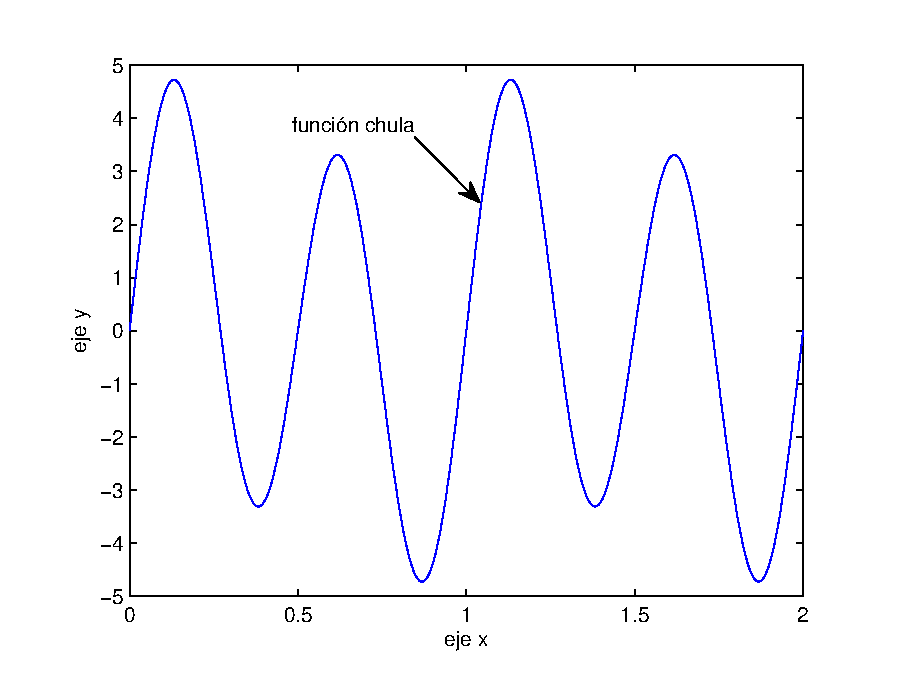
\includegraphics[scale=0.5]{ejemplo.eps}
\caption{Figurita ejemplo}
\label{fig:figurita-ejemplo}
\end{figure}

La forma de incluir la figura es simple:

\begin{lstlisting}[language={[LaTeX]TeX},frame=none,numbers=none]
\begin{figure}
\centering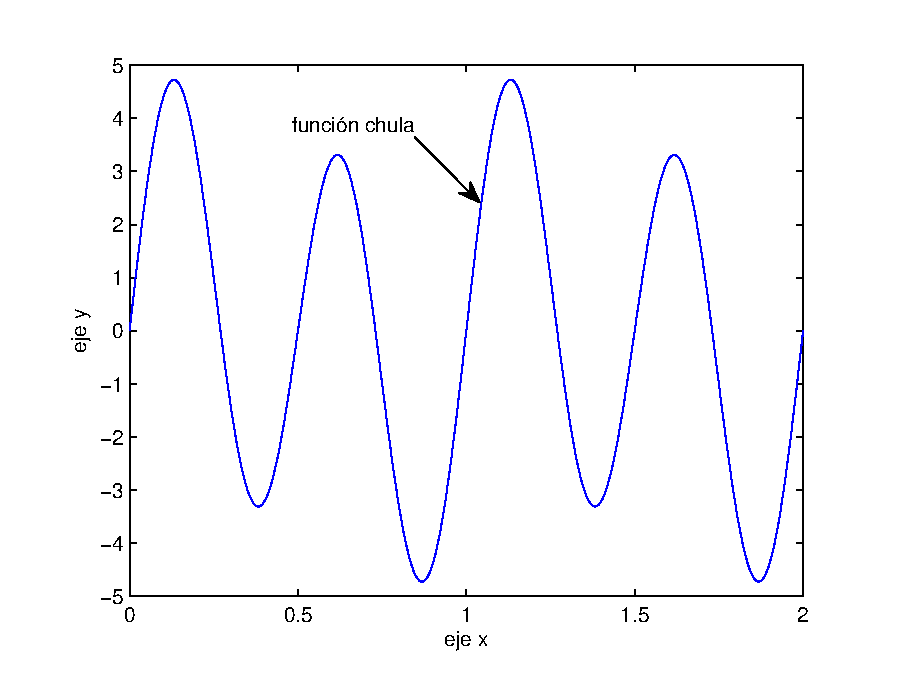
\includegraphics[width=6cm]{ejemplo.eps}
\caption{Figurita ejemplo}
\label{fig:figurita-ejemplo}
\end{figure}
\end{lstlisting}

El entorno \texttt{figure} crea un cuadro flotante, con todo el contenido de la figura, que \LaTeX{} coloca en el sitio menos malo.  La \texttt{caption} es el pie de la figura y la \texttt{label} es la etiqueta que nos permitirá referirnos a ella en el texto (con la orden \texttt{ref}).

\LaTeX{} utiliza un algoritmo nada evidente para colocar las figuras de manera que sea estéticamente agradable.  Pero tú puedes influir en las preferencias de colocación.  El entorno \texttt{figure} tiene un parámetro opcional entre corchetes que indica las opciones de colocación.  Por defecto es \texttt{[tbp]}, que equivale a \emph{top, bottom, page}.  Eso quiere decir que intenta primero ponerla a comienzo de página.  Si no lo consigue, al final de una página.  Y si así tampoco lo consigue, en una página entera, solo para la figura.  En este ejemplo utilizo las opciones \texttt{[hbtp]} para que intente la secuencia \emph{here, bottom, top, page}.  En este caso prefiero que la ponga debajo antes que arriba, para que no aparezca en una sección anterior.

Con \LaTeX{} puedes conseguir que las figuras no se muevan en absoluto, pero eso deja documentos extremadamente descompensados.  No lo hagas nunca.  Es mejor mover ligeramente la figura en el texto o incluso re-escribir parte del texto, antes de forzar la posición.  De todas formas, si no me quieres hacer caso, en la fig.~\ref{fig:figurita-ejemplo-2}  tienes un ejemplo que fuerza la posición.

\begin{figure}[H]
\centering
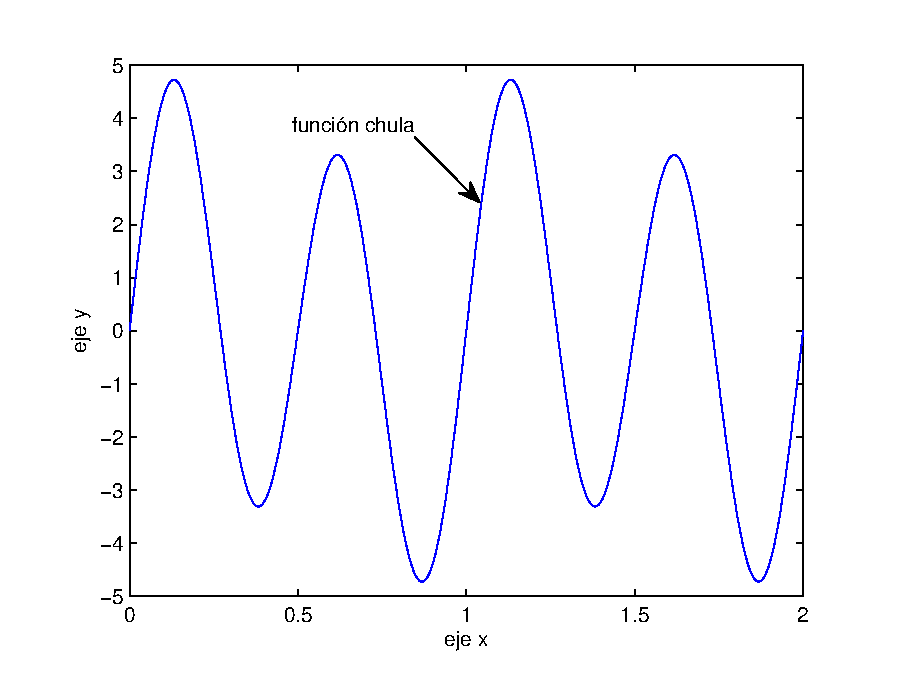
\includegraphics[scale=0.5, angle=15]{ejemplo.eps}
\caption{Figurita ejemplo 2}
\label{fig:figurita-ejemplo-2}
\end{figure}

Para poder poner figuras que no son de elaboración propia es necesario primero obtener permiso del autor y, además, añadir la fuente al pie de foto. Hay muchas guías de estilo que explican en detalle cómo hacerlo. Por ejemplo, la \emph{American Psychological Association} tiene un \href{https://www.lib.sfu.ca/help/research-assistance/format-type/online-images/citing#citing-images-in-apa}{capítulo específico de su manual de publicaciones}.  El manual de la APA se usa extensivamente en todo tipo de literatura científica.

\begin{figure}[htb]
\centering
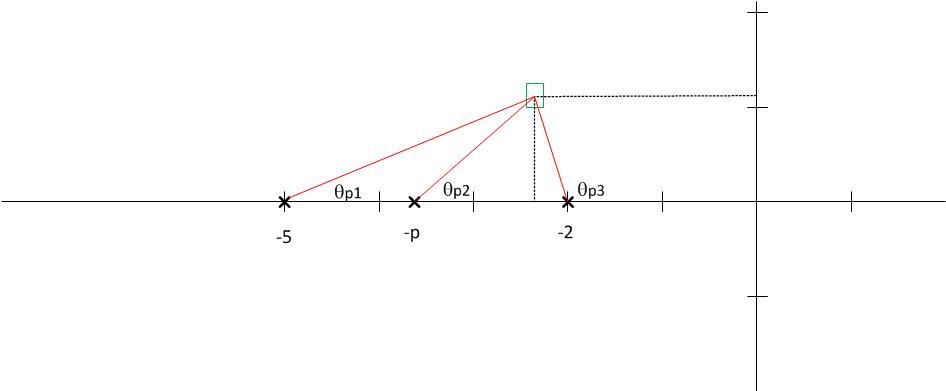
\includegraphics[scale = 0.5]{ejemplo2.jpg}
\caption{Figurita ejemplo 3. Extraída de la plantilla de TFG de Fernando Castillo. \copyright 2018 Fernando Castillo. Reproducida con permiso.}
\label{fig:figura-ejemplo-3}
\end{figure}

\warning{Fíjate bien.  No se citan las imágenes como si se tratara de referencias bibliográficas.  No debe haber pie de página (orden \texttt{footnote}) ni cita (orden \texttt{cite}) en un pie de foto (\texttt{caption}).  La atribución de la obra debe estar al mismo nivel que la obra usada.  Por eso debe atribuirse completamente en el pie de foto.  Si no te gusta como queda haz tus propias imágenes.}

Se puede controlar el escalado de la imagen y el ángulo de forma muy sencilla, con las opciones de la orden \texttt{includegraphics}.  En la fig.~\ref{fig:figura-ejemplo-3} se muestra un ejemplo de figura escalado a un 30\%.  La orden \texttt{includegraphics} ajusta los parámetros de la imagen para mantener la relación de aspecto original, si esto es posible.  Esto hace que podamos especificar simplemente el ancho o el alto deseado, que va a ser lo más habitual.  En mi opinión, las opciones más frecuentes de \texttt{includegraphics} son, por orden:

\begin{figure}
\centering
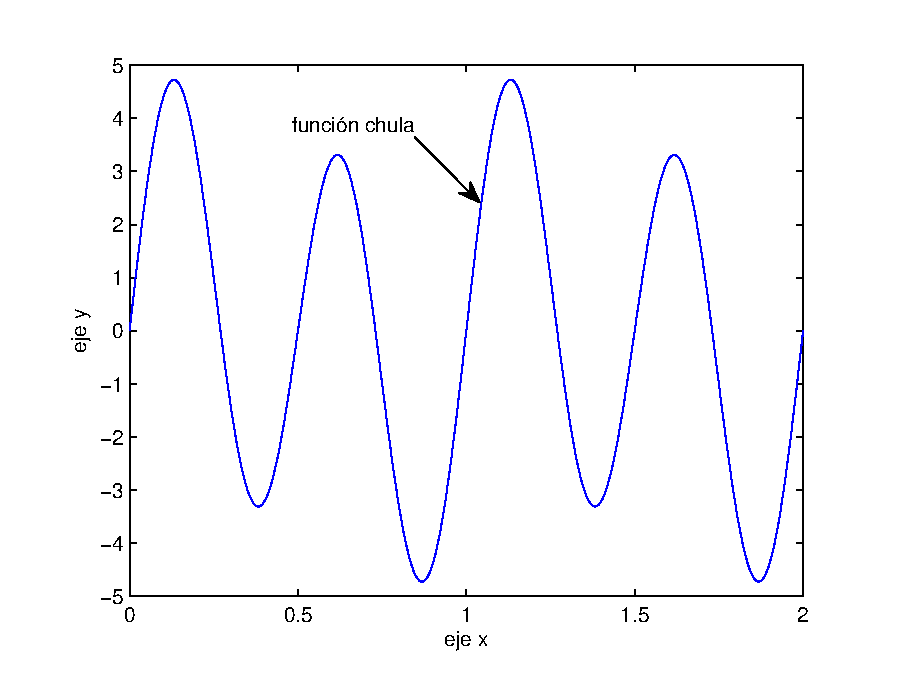
\includegraphics[width=\textwidth]{ejemplo.eps}
\caption{Figura ejemplo que ocupa todo el ancho del texto.}
\label{fig:figura-ejemplo-4}
\end{figure}

\begin{description}
\item[\texttt{width}]  Fija el ancho de la imagen.  Puede ser un tamaño absoluto en centímetros (\texttt{cm}), milímetros (\texttt{mm}) o puntos PostScript (\texttt{pt}).  Por ejemplo,  \verb|width=1.5cm|.  También puede ser un tamaño relativo a cualquier medida del documento.  Por ejemplo, \verb|width=0.5\textwidth| sería una figura que ocupe la mitad del ancho del texto.

\item[\texttt{height}] Fija la altura de la imagen.  Es similar a \texttt{width} pero con la altura.  Se puede especificar tanto altura como anchura, de manera que se modifica la relación de aspecto original.

\item[\texttt{scale}] Utiliza un factor de escala para la imagen.  Puede ser mayor de 1 para ampliar la imagen.

\item[\texttt{angle}] Gira la imagen un número de grados determinado.  Si el número es negativo el giro es en sentido horario.  Si es positivo el giro es antihorario.
\end{description}


En la fig.~\ref{fig:figura-angulo-30} se muestra un ejemplo de figura girada 30.

\begin{figure}[btp]
\centering
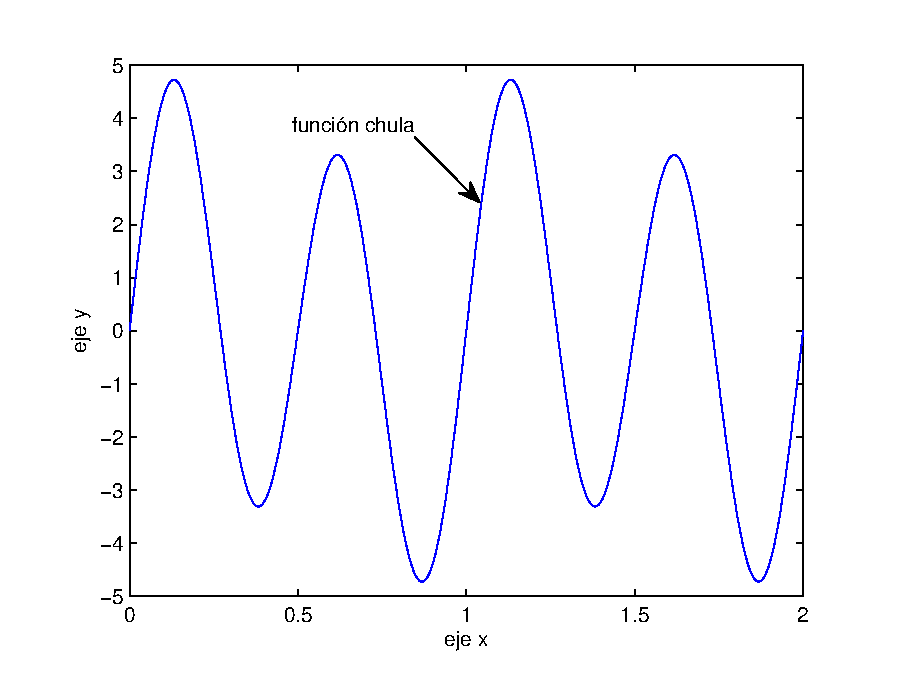
\includegraphics[width=.3\textwidth,angle=-30]{ejemplo.eps}
\caption{Figura ejemplo de rotación.}
\label{fig:figura-angulo-30}
\end{figure}

Una característica interesante del entorno \texttt{figure} es que permite definir sub-figuras con la orden \texttt{subfigure} o el entorno del mismo nombre.  La colocación de las sub-figuras es prácticamente automática.  Un ejemplo puede verse en la figura~\ref{fig:matriz-figuras}.

\begin{figure}[htbp]
\centering
\subfigure[figurita1]{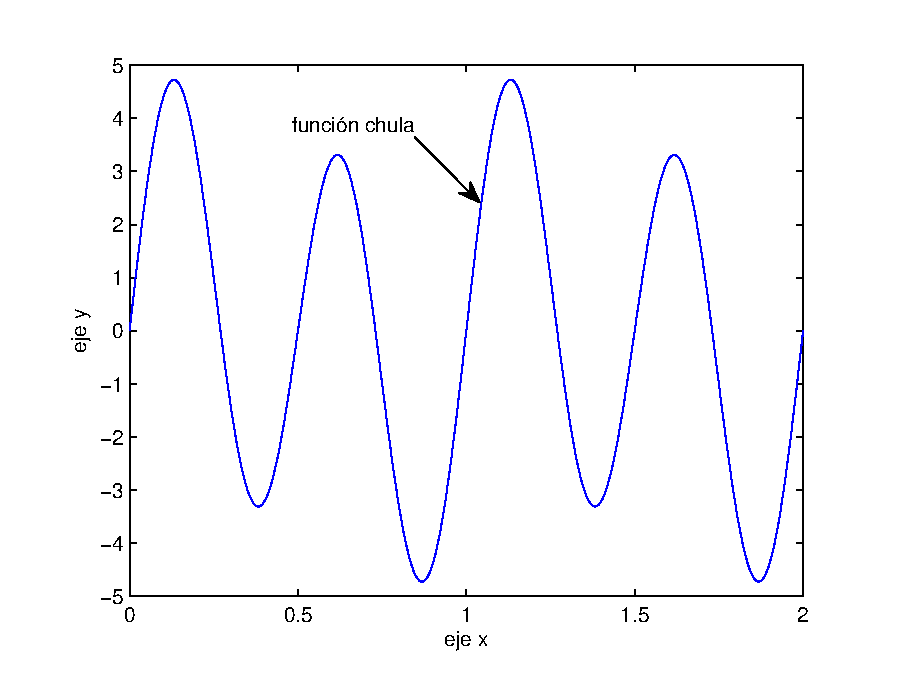
\includegraphics[width=40mm]{ejemplo.eps}}
\subfigure[figurita2]{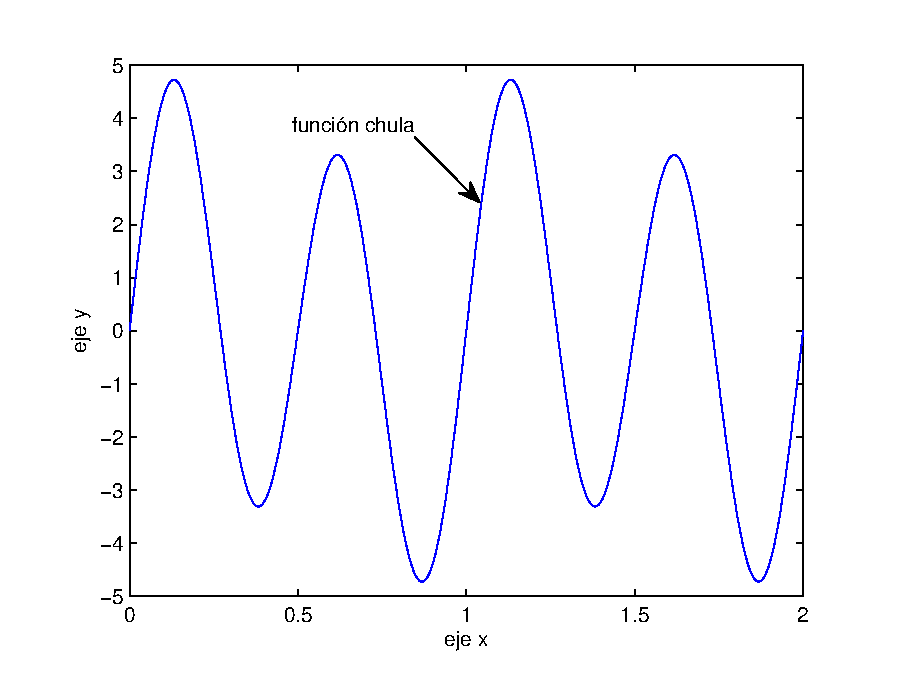
\includegraphics[width=40mm]{ejemplo.eps}}
\subfigure[figurita3]{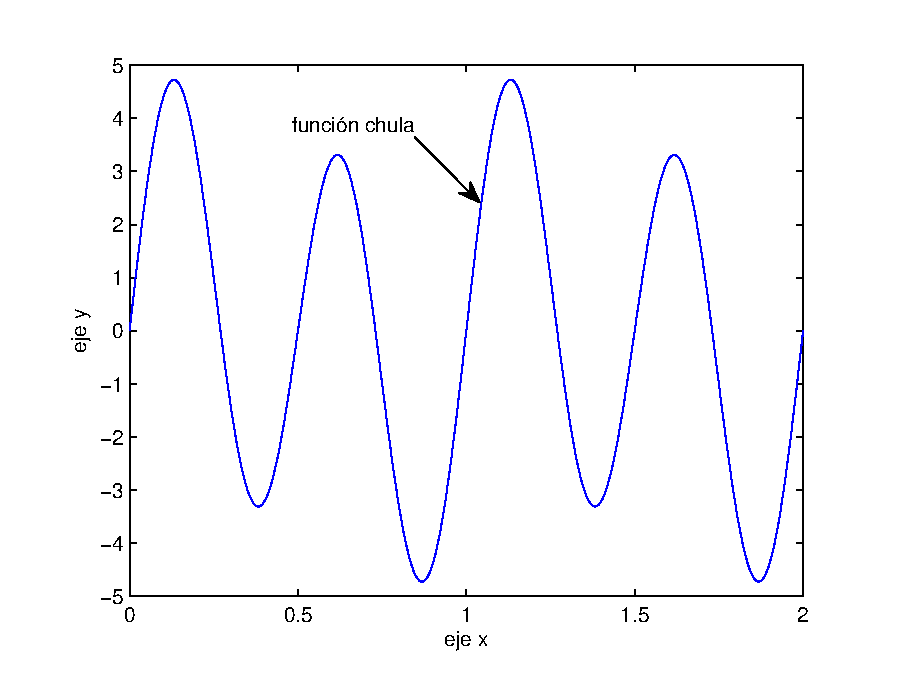
\includegraphics[width=80mm]{ejemplo.eps}}
\caption{Matriz de figuras} 
\label{fig:matriz-figuras}
\end{figure}

Una subfigura puede referenciarse a partir de la referencia a la figura.  Por ejemplo, la figura~\ref{fig:matriz-figuras}(a) es igual que la figura~\ref{fig:matriz-figuras}(b). Sin embargo, cuando las figuras son muy complejas, es posible que se prefieran esquemas más automáticos.  En \href{https://tex.stackexchange.com/questions/181225/how-to-reference-to-subfigure-in-latex}{StackExchange} encontrarás soluciones a éste y otros problemas con mucha facilidad.

En general, he tratado de mantener un compromiso entre el número de características incluidas y la facilidad de uso de la plantilla.  Las figuras muy complejas es algo que prefiero evitar, así que en el estilo de la plantilla no incorpora los paquetes \texttt{subcaption} y \texttt{cleveref}.
